\appendix
\providecommand{\multirow}[3]{#3}

\section{Dataset and Fine-Tuning}\label{app:dataset}
The pipeline is evaluated on a basketball clip from the Sanbapolis facility, recorded by
three synchronised cameras (cam\_13, cam\_2, cam\_4).
The clip spans 525 frames at 25\,fps (about 21\,s).
Camera intrinsics are provided, and ground-truth 2D bounding boxes are annotated on every fifth frame for evaluation.

The detector is fine-tuned on a separate dataset from the same game, covering different actions,
disjoint from the evaluation clip. Training starts from YOLO26m weights and runs for up to 300 epochs (early stopping,
patience 30) at $1280$\,px input and batch size 4.

\section{Pipeline Parameters}\label{app:parameters}
The following tables list the parameters used at each stage of the pipeline: MOG2
background subtraction (Table~\ref{tab:par-mog2}), YOLO detection and NMS
(Table~\ref{tab:par-yolo}), tracking (Table~\ref{tab:par-tracking}), and 3D geometry
(Table~\ref{tab:par-geometry}).

\begin{table}[H]
    \centering
    \small
    \begin{minipage}[t]{0.48\textwidth}
        \centering
        \caption{MOG2 background subtraction and preprocessing.}
        \label{tab:par-mog2}
        \begin{tabular}{lr}
            \toprule
            Parameter & Value \\
            \midrule
            Learning rate            & $-1$ (adaptive) \\
            Detect shadows           & off \\
            CLAHE clip limit         & 6.0 \\
            CLAHE tile grid          & $8\times8$ \\
            Min.\ blob area (px$^2$) & 500 \\
            Max.\ blob area (px$^2$) & 10000 \\
            \bottomrule
        \end{tabular}
    \end{minipage}
\hfill
    \begin{minipage}[t]{0.48\textwidth}
        \centering
        \caption{Geometry: smoothing and triangulation.}
        \label{tab:par-geometry}
        \begin{tabular}{lr}
            \toprule
            Parameter & Value \\
            \midrule
            \multicolumn{2}{l}{\textit{2D trajectory smoothing}} \\
            \quad Max.\ interpolated gap (frames) & 5 \\
            \quad EMA weight $\alpha$              & 0.5 \\
            \multicolumn{2}{l}{\textit{Triangulation}} \\
            \quad Ground inlier gate (mm)     & 600 \\
            \quad Ball reprojection gate (px) & 30 \\
            \quad Minimum views               & 2 \\
            \multicolumn{2}{l}{\textit{3D trajectory smoothing}} \\
            \quad Max.\ join gap (frames)       & 5 \\
            \quad Mahalanobis gate ($\chi^2$)   & 11.345 \\
            \quad Position noise std (mm)       & 30 \\
            \quad Velocity noise std (mm/frame) & 60 \\
            \quad Measurement noise std (mm)    & 80 \\
            \bottomrule
        \end{tabular}
    \end{minipage}
\end{table}

\begin{table}[H]
\centering
\small
\begin{minipage}[t]{0.48\textwidth}
\centering
\caption{YOLO detection and NMS.}
\label{tab:par-yolo}
\begin{tabular}{lr}
\toprule
Parameter & Value \\
\midrule
\multicolumn{2}{l}{\textit{Single-pass YOLO}} \\
\quad Confidence threshold      & 0.3 \\
\quad Inference size (px)       & 640 \\
\quad Built-in NMS IoU          & 0.45 \\
\multicolumn{2}{l}{\textit{Two-pass fine-tuned}} \\
\quad Player inference size (px) & 1280 \\
\quad Ball inference size (px)   & 1600 \\
\quad Ball confidence            & 0.2 \\
\quad Player low-conf band       & 0.15 \\
\multicolumn{2}{l}{\textit{Class-agnostic merge NMS}} \\
\quad IoU suppression threshold & 0.75 \\
\bottomrule
\end{tabular}
\end{minipage}
\hfill
\begin{minipage}[t]{0.48\textwidth}
\centering
\caption{Tracking (SORT and DeepSORT).}
\label{tab:par-tracking}
\begin{tabular}{lr}
\toprule
Parameter & Value \\
\midrule
\multicolumn{2}{l}{\textit{SORT}} \\
\quad Max.\ IoU distance        & 0.8 \\
\quad Max.\ age (frames)        & 60 \\
\quad Confirmation hits         & 2 \\
\multicolumn{2}{l}{\textit{DeepSORT}} \\
\quad Max.\ IoU distance        & 0.7 \\
\quad Max.\ appearance distance & 0.2 \\
\quad Max.\ age (frames)        & 60 \\
\quad Confirmation hits         & 2 \\
\quad Feature budget per track  & 100 \\
\quad Coast age (frames)        & 5 \\
\quad Coast max.\ IoU           & 0.3 \\
\quad Resurrection window (frames) & 150 \\
\quad Resurrection max.\ distance  & 0.25 \\
\multicolumn{2}{l}{\textit{Appearance (OSNet)}} \\
\quad Input size (px)           & $256\times128$ \\
\quad Embedding dimension       & 512 \\
\bottomrule
\end{tabular}
\end{minipage}
\end{table}

\section{Detailed Results}\label{app:results}

This section reports per-camera detection (Table~\ref{tab:app-detection}), tracking
(Table~\ref{tab:app-tracking}), and 3D geometry errors
(Table~\ref{tab:app-geometry-errors}).

\begin{table}[H]
\centering
\caption{Detection results across cameras (IoU threshold $=0.5$).}
\label{tab:app-detection}
\small
\begin{tabular}{llrrrr}
\toprule
Method & Camera & Precision & Recall & $F_1$ & Mean IoU \\
\midrule
\multirow{3}{*}{MOG2}
  & cam\_13 & 0.471 & 0.262 & 0.337 & 0.651 \\
  & cam\_2  & 0.345 & 0.408 & 0.374 & 0.663 \\
  & cam\_4  & 0.328 & 0.293 & 0.309 & 0.700 \\
\midrule
\multirow{3}{*}{YOLO pre-trained}
  & cam\_13 & 0.851 & 0.617 & 0.716 & 0.754 \\
  & cam\_2  & 0.858 & 0.778 & 0.816 & 0.782 \\
  & cam\_4  & 0.922 & 0.801 & 0.857 & 0.808 \\
\midrule
\multirow{3}{*}{YOLO fine-tuned}
  & cam\_13 & 0.872 & 0.732 & 0.796 & 0.758 \\
  & cam\_2  & 0.835 & 0.761 & 0.796 & 0.757 \\
  & cam\_4  & 0.923 & 0.822 & 0.870 & 0.796 \\
\bottomrule
\end{tabular}
\end{table}

\begin{table}[H]
\centering
\caption{Tracking metrics: identity (IDP, IDR, IDF1) and HOTA (IoU threshold $=0.5$).}
\label{tab:app-tracking}
\footnotesize
\setlength{\tabcolsep}{4.5pt}
\begin{tabular}{llrrrrrrr}
\toprule
Tracker & Camera & IDP & IDR & IDF1 & HOTA & DetA & AssA & LocA \\
\midrule
\multirow{3}{*}{SORT}
  & cam\_13 & 0.660 & 0.514 & 0.590 & 0.438 & 0.484 & 0.398 & 0.797 \\
  & cam\_2  & 0.743 & 0.607 & 0.668 & 0.517 & 0.515 & 0.522 & 0.794 \\
  & cam\_4  & 0.768 & 0.605 & 0.679 & 0.542 & 0.575 & 0.514 & 0.829 \\
\midrule
\multirow{3}{*}{DeepSORT}
  & cam\_13 & 0.588 & 0.533 & 0.569 & 0.434 & 0.469 & 0.405 & 0.769 \\
  & cam\_2  & 0.617 & 0.603 & 0.610 & 0.480 & 0.453 & 0.511 & 0.761 \\
  & cam\_4  & 0.670 & 0.605 & 0.638 & 0.521 & 0.553 & 0.495 & 0.798 \\
\bottomrule
\end{tabular}
\end{table}

\begin{table}[H]
\centering
\caption{3D geometry errors: reprojection of triangulated points and trajectory error of
projected tracks. Mean, Median, RMSE, ADE, FDE, and MTE are in mm; Acc columns are
fractions at 25, 50, 100\,mm. Fragment counts are 2, 5, 5 for cam\_13, cam\_2, cam\_4.}
\label{tab:app-geometry-errors}
\footnotesize
\setlength{\tabcolsep}{2pt}
\begin{tabular}{lrrrrrrrrr}
\toprule
& \multicolumn{6}{c}{Reprojection error} & \multicolumn{3}{c}{Trajectory error} \\
\cmidrule(lr){2-7}\cmidrule(lr){8-10}
Camera & Mean & Median & RMSE & Acc@25 & Acc@50 & Acc@100 & ADE & FDE & MTE \\
\midrule
cam\_13 & 499.6 & 300.5 &  844.9 & 0.087 & 0.134 & 0.219 &  9976.1 &  8503.9 & 10662.2 \\
cam\_2  & 772.5 & 459.6 & 1378.8 & 0.023 & 0.038 & 0.076 &  3984.4 &  5098.8 &  4373.3 \\
cam\_4  & 395.3 & 176.0 &  905.4 & 0.188 & 0.247 & 0.359 &  8636.7 &  7238.4 &  8739.9 \\
\bottomrule
\end{tabular}
\end{table}

\section{Qualitative Outputs}\label{app:figures}
The figures below are the per-stage visual outputs produced by the pipeline notebook on
cam\_13.

\begin{figure}[H]
  \centering
  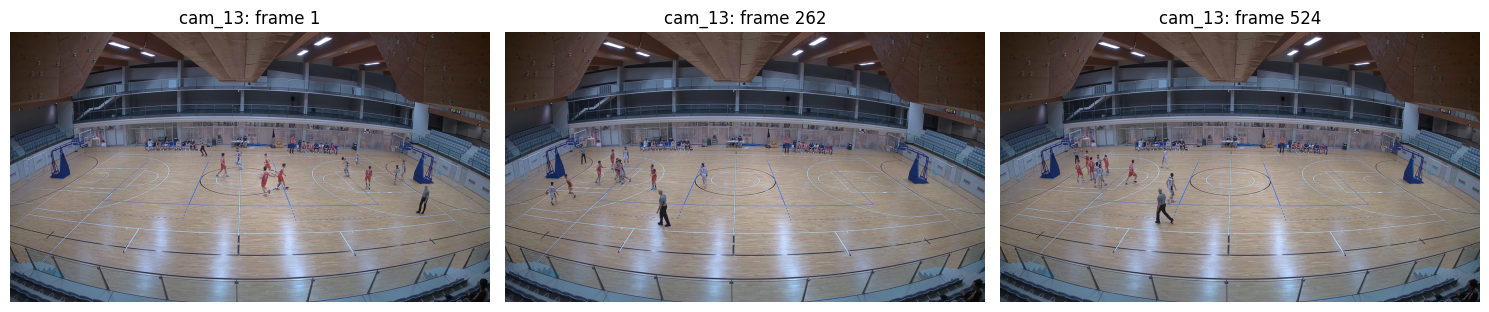
\includegraphics[width=\linewidth]{../media/appendix/01_open_video_and_read_frames.png}
  \caption{Raw input frame.}
\end{figure}

\begin{figure}[H]
  \centering
  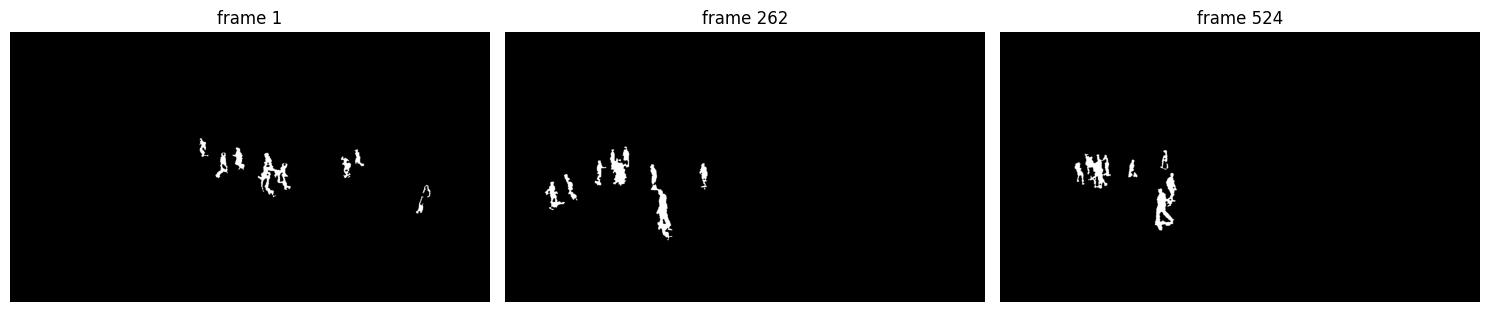
\includegraphics[width=\linewidth]{../media/appendix/02_inspect_mog2_detections.png}
  \caption{MOG2 foreground mask.}
\end{figure}

\begin{figure}[H]
  \centering
  
\includegraphics[width=\linewidth]{../media/appendix/03_inspect_mog2_detections.png}
  \caption{MOG2 detections overlaid on the frame.}
\end{figure}

\begin{figure}[H]
  \centering
  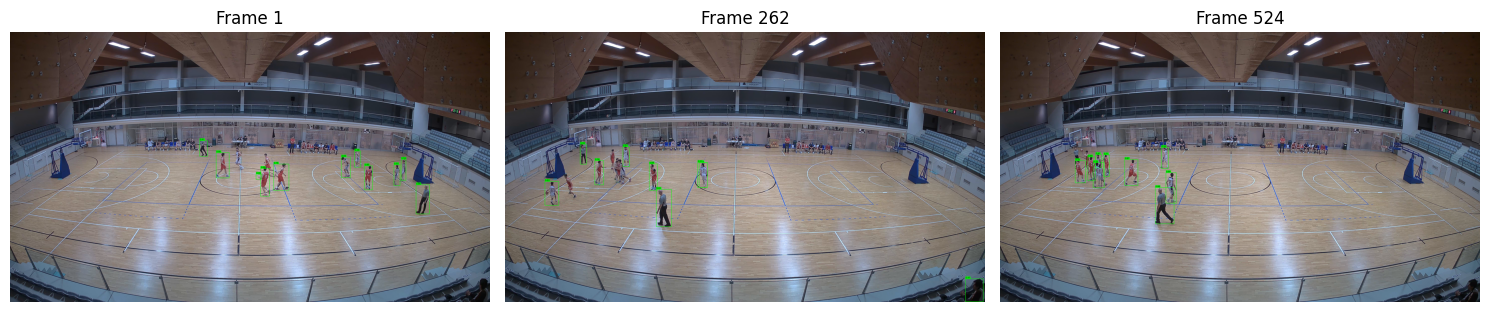
\includegraphics[width=\linewidth]{../media/appendix/04_inspect_yolo_detections.png}
  \caption{Pre-trained YOLO26 detections.}
\end{figure}

\begin{figure}[H]
  \centering
  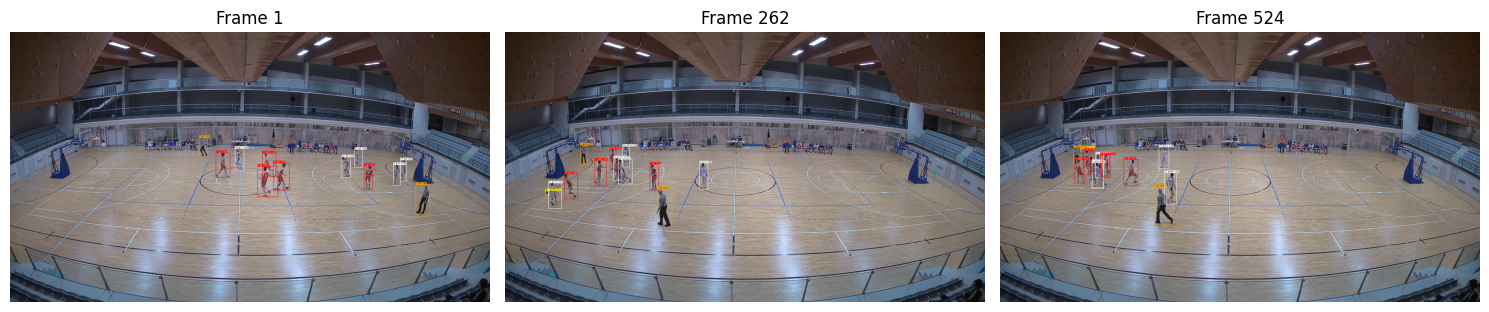
\includegraphics[width=\linewidth]{../media/appendix/10_inspect_resolved_labels.png}
  \caption{DeepSORT tracks after smoothing and label resolution.}
\end{figure}

\begin{figure}[H]
  \centering
  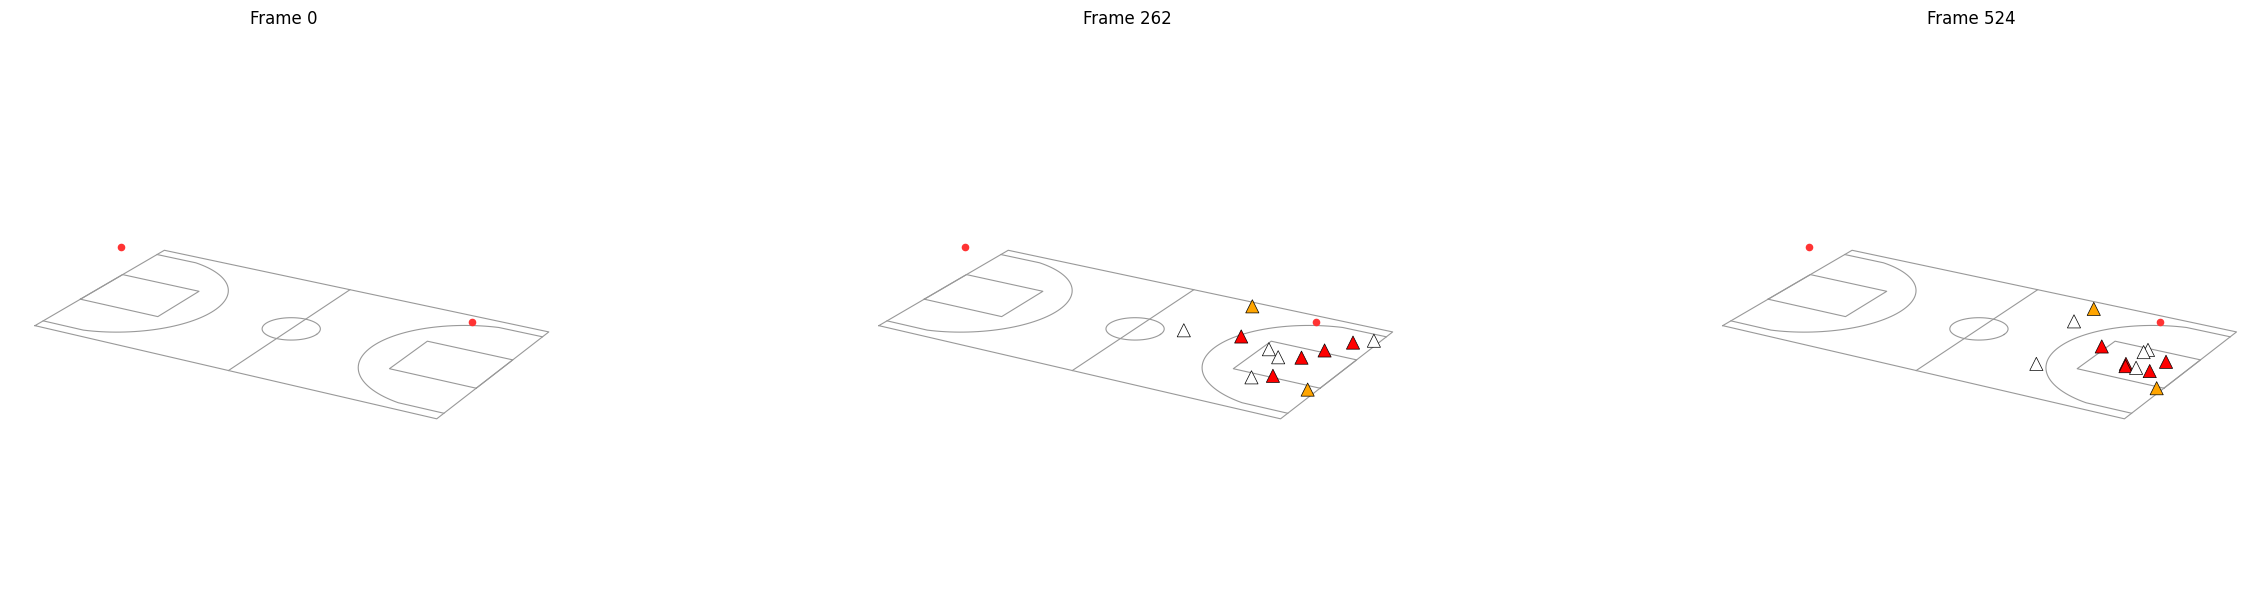
\includegraphics[width=\textwidth]{../media/appendix/12_inspect_smoothed_3d_reconstructions.png}
  \caption{Smoothed 3D reconstruction.}
\end{figure}
